\documentclass[10pt]{dokument-ppi}

\begin{document}


\Cwiczenie{5}
\Tytul{Dokument modelu jakości}
\Data{2012-12-29}
\Wersja{1.0}
\Autorzy{ŁG, DG, AO, MS}
\MakeDokumentMeta


\section{Wprowadzenie}

Poniższy dokument został przygotowany w oparciu o model kontroli jakości
oprogramowania \textsc{FURPS}.


\section{Wymagania}

\subsection{Funkcjonalność}

\subsubsection{Bezpieczeństwo}
\begin{requirement}
    \desc%
        Korzystanie z API, umożliwiającego zarządzenie materiałami przez
        partnerów będzie wymagało uwierzytelnienia. Zabezpiecza to system przed
        nieporządanymi i niewiarygodnymi źródłami danych.
    \metric%
        Ilość etapów uwierzytelnienia.
    \tool%
        Lista kontrolna.
    \scale%
        \emph{1} --- Brak uwierzylnienia.\\
        \emph{3} --- Uwierzylnienie jednostopniowe.\\
        \emph{5} --- Uwierzylnienie dwustopniowe.
    \weight 5
\end{requirement}

\subsubsection{Lokalizacja}
\begin{requirement}
    \desc%
        Wielojęzyczność zapewniająca możliwość korzystania z systemu przez osoby
        nieznające języka natywnego.
    \metric%
        Ilość obsługiwanych języków.
    \tool%
        Lista kontrolna.
    \scale%
        \emph{1} --- Dostępna tylko wersja w języku polskim.\\
        \emph{3} --- Dostępna wersja w języku polskim oraz angielskim.\\
        \emph{5} --- Obsługa więcej niż dwóch języków, z możliwoścą łatwego
            dodania nowych lokalizacji.
    \weight 2
\end{requirement}

\subsubsection{Pomoc}
\begin{requirement}
    \desc%
        Samouczki dla użytkowników aplikacji mobilnej. Dokumentacja techniczna
        API dla organizatorów współpracujących.
    \metric%
        Ilość dostępnych materiałów szkoleniowych.
    \tool%
        Lista kontrolna.
    \scale%
        \emph{1} --- Brak materiałów.\\
        \emph{2} --- Dokumentacja techniczna API dla współpracujących
            organizatorów.\\
        \emph{3} --- Samouczek w aplikacji mobilnej. Dokumentacja techniczna API
            dla współpracujących organizatorów.\\
        \emph{5} --- Samouczek w aplikacji mobilnej. Dokumentacja techniczna API
            oraz szkolenia dla współpracujących organizatorów.
    \weight 2
\end{requirement}

\subsubsection{Drukowanie}
\begin{requirement}
    \desc%
        Wyświetlanie informacji zwrotnych użytkownikowi aplikacji mobilnej.
        Kompletność informacji, które otrzymuje od serwera.
    \metric%
        Kompletność informacji zwrotnych i dostępność komunikatów o błędach.
    \tool%
        Lista kontrolna.
    \scale%
        \emph{1} --- Aplikacja mobilna nie wyświetla informacji zwrotnych.\\
        \emph{2} --- Aplikacja mobilna wyświetla częściowo informacje zwrotne,
            bez komunikatów o błędach.\\
        \emph{3} --- Aplikacja mobilna wyświetla kompletne informacje zwrotne,
            bez komunikatów o błędach.\\
        \emph{5} --- Aplikacja mobilna wyświetla kompletne informacje zwrotne
        oraz komunikaty o błędach.
    \weight 5
\end{requirement}

\subsubsection{Raportowanie}
\begin{requirement}
    \desc%
        Zbieranie logów systemowych i ich przetwarzanie. Informacje dotyczące
        liczby użytkowników korzystających z systemu oraz sposobu, w jaki z
        niego korzystają (wyszukiwanie obrazów, zakup biletów). Logi powinny
        zawierać także informacje o występowaniu awarii.
    \metric%
        Dostępność statystyk dla współpracujących organizatorów.
    \tool%
        Lista kontrolna.
    \scale%
        \emph{1} --- Brak logów systemowych.\\
        \emph{2} --- Informacje o liczbie użytkowników, sposobie użycia aplikacji oraz błędach.\\
        \emph{3} --- Informacje o liczbie użytkowników, sposobie użycia aplikacji oraz błędach. Dodatkowo możliwość generowania raportów z dowolnego okresu.\\
        \emph{5} --- Informacje o liczbie użytkowników, sposobie użycia aplikacji oraz błędach. Dodatkowo możliwość generowania raportów z dowolnego okresu. Statystyki obrazują stan z maksymalnie jednej godziny od zgłoszenia zapytania o wygenerowanie statystyk.
    \weight%
        4. Statystyki, jeśli są zadowalające, pozwalają pozyskać nowych
        współpracowników.
\end{requirement}

\subsubsection{Zarządzanie}
\begin{requirement}
    \desc%
        Możliwość zarządzania informacjami w bazie wydarzeń. Dodawanie, edycja, usuwanie i wyszukiwanie wydarzeń.
    \metric%
        Dostępność funkcji obsługi wydarzeń.
    \tool%
        Lista kontrolna.
    \scale%
        \emph{1} --- Wyszukiwanie wydarzeń.\\
        \emph{2} --- Wyszukiwanie, dodawanie wydarzeń.\\
        \emph{4} --- Wyszukiwanie, dodawanie, edycja wydarzeń.\\
        \emph{5} --- Wyszukiwanie, dodawanie, edycja i usuwanie wydarzeń.
    \weight%
        4
\end{requirement}


\subsection{Użyteczność}

\subsubsection{Intuicyjność}
\begin{requirement}
    \desc%
        Prostota obsługi i łatwy dostęp do funkcjonalności aplikacji mobilnej.
    \metric%
        Ankietyzacja wybranej grupy użytkowników.
    \tool%
        Histogram.
    \scale%
        \emph{1} --- Poniżej 50\% ankietowanych uznało interfejs za intuicyjny.\\
        \emph{2} --- Od 50\% do 60\% ankietowanych uznało interfejs za intuicyjny.\\
        \emph{3} --- Od 60\% do 70\% ankietowanych uznało interfejs za intuicyjny.\\
        \emph{4} --- Od 70\% do 80\% ankietowanych uznało interfejs za intuicyjny.\\
        \emph{5} --- Powyżej 80\% ankietowanych uznało interfejs za intuicyjny.
    \weight%
        5
\end{requirement}

\subsubsection{Estetyka}
\begin{requirement}
    \desc%
        Wygląd interfejsu użytkownika.
    \metric%
        Ankietyzacja wybranej grupy użytkowników.
    \tool%
        Histogram.
    \scale%
        \emph{1} --- Poniżej 50\% ankietowanych uznało aplikację za estetyczną.\\
        \emph{2} --- Od 50\% do 60\% ankietowanych uznało aplikację za estetyczną.\\
        \emph{3} --- Od 60\% do 70\% ankietowanych uznało aplikację za estetyczną.\\
        \emph{4} --- Od 70\% do 80\% ankietowanych uznało aplikację za estetyczną.\\
        \emph{5} --- Powyżej 80\% ankietowanych uznało aplikację za estetyczną.
    \weight%
        3
\end{requirement}


\subsection{Niezawodność}

\subsubsection{Dokładność}
\begin{requirement}
    \metric*%
        Procent poprawnie rozpoznanych zdjęć plakatów.
    \tool%
        Histogram.
    \scale%
        \emph{1} --- Poniżej 50\%.\\
        \emph{2} --- Od 50\% do 60\%.\\
        \emph{3} --- Od 60\% do 80\%.\\
        \emph{4} --- Od 80\% do 95\%.\\
        \emph{5} --- Powyżej 95\%.
    \weight%
        5
\end{requirement}

\subsubsection{Dostępność}
\begin{requirement}
    \metric*%
        Procent czasu bezawaryjnej pracy serwera.
    \tool%
        Histogram.
    \scale%
        \emph{1} --- Poniżej 70\%.\\
        \emph{2} --- Od 70\% do 85\%.\\
        \emph{3} --- Od 85\% do 95\%.\\
        \emph{4} --- Od 95\% do 99\%.\\
        \emph{5} --- Powyżej 99\%.
    \weight%
        5
\end{requirement}

\subsubsection{Mechanizmy naprawcze}
\begin{requirement}
    \desc%
        Dostępność mechanizmów i procedur pozwalających uniknąć lub naprawić
        awarie systemu. Na przykład uszkodzenie dysku czy niedobór pamięci.
    \metric%
        Liczba dostępnych mechanizmów.
    \tool%
        Lista kontrolna.
    \scale%
        \emph{1} --- System nie posiada odpowiednich mechanizmów.\\
        \emph{3} --- System potrafi zareagować automatycznie na 50\% przewidzianych awarii.\\
        \emph{5} --- System potrafi zareagować automatycznie na 80\% przewidzianych awarii.
    \weight%
        5
\end{requirement}


\subsection{Wydajność}

\subsubsection{Czas odpowiedzi}
\begin{requirement}
    \desc%
        Czas od wysłania zdjęcia przez użytkownika do uzyskania informacji
        zwrotnej o wydarzeniu.
    \metric%
        Liczba sekund między wysłaniem żądania a otrzymaniem odpowiedzi.
    \tool%
        Histogram.
    \scale%
        \emph{1} --- Dłuższy niż 15 sekund.\\
        \emph{2} --- Od 10 do 15 sekund.\\
        \emph{3} --- Od 6 do 9 sekund.\\
        \emph{4} --- Od 3 do 6 sekund.\\
        \emph{5} --- Poniżej 3 sekund.
    \weight%
        3
\end{requirement}

\subsubsection{Przepustowość}
\begin{requirement}
    \desc%
        Maksymalna możliwa liczba porównywanych obrazów w przeciągu sekundy.
    \metric%
        Liczba obrazów porównywanych w przeciągu sekundy.
    \tool%
        Histogram.
    \scale%
        \emph{1} --- Poniżej 3 tys.\\
        \emph{2} --- Od 3 tys. do 7 tys.\\
        \emph{3} --- Od 7 tys. do 9 tys..\\
        \emph{4} --- Od 9 tys. do 10 tys.\\
        \emph{5} --- Powyżej 10 tys.
    \weight%
        5
\end{requirement}

\subsubsection{Czas naprawy}
\begin{requirement}
    \desc%
        Jak szybko system wraca do normalnego trybu pracy po wystąpieniu
        krytycznej awarii.
    \metric%
        Liczba godzin od momentu wystąpienia awarii do usunięcia jej skutków.
    \tool%
        Histogram.
    \scale%
        \emph{1} --- Dłużej niż 24 godziny.\\
        \emph{3} --- Od 12 do 24 godzin.\\
        \emph{5} --- Poniżej 12h.
    \weight%
        5
\end{requirement}


\subsection{Wsparcie}

\subsubsection{Łatwość testowania}
\begin{requirement}
    \desc%
        Polega na określeniu kompletności dokumentacji i zaawansowania
        procesu testowania. Automatyczny zestaw testów, o wysokim
        pokryciu, ułatwia zarządzanie i wprowadzanie zmian do systemu.
    \metric%
        Łatwość przeprowadzania testów.
    \tool%
        Lista kontrolna.
    \scale%
        \emph{1} --- Brak automatycznych testów i niekompletność dokumentacji.\\
        \emph{2} --- System posiada kompletną dokumentację, ale testy muszą zostać utworzone od podstaw.\\
        \emph{4} --- Automatyczne testy dla krytycznych funkcji systemu.\\
        \emph{5} --- Automatyczne testy dla wszystkich funkcji systemu.
    \weight%
        5
\end{requirement}

\subsubsection{Skalowalność}
\begin{requirement}
    \desc%
        Możliwe jest, że liczba wysyłanych zapytań spowoduje przeciążenie
        systemu. Można zapobiec tym awariom zwiększając możliwości obliczeniowe
        systemu.
    \metric%
        Wpływ na ciągłość pracy systemu i łatwość zwiększenia możliwości
        systemu.
    \tool%
        Lista kontrolna.
    \scale%
        \emph{1} --- Wymagana jest zmiana architektury i kodu systemu.\\
        \emph{3} --- Wymagane jest ręczne zarządzenie instancjami serwerów przez zespół projektowy. Bez konieczności modyfikacji kodu systemu.\\
        \emph{5} --- System automatycznie zarządza liczbą aktywnych instacji serwerów zależnie od obciążenia systemu.
    \weight%
        4
\end{requirement}

\subsubsection{Łatwość utrzymania}
\begin{requirement}
    \metric*%
        Stopień wpływu wprowadzania aktualizacji oprogramowania na działanie
        systemu.
    \tool%
        Lista kontrolna.
    \scale%
        \emph{1} --- Dowolna aktualizacja wymaga przerwy w działaniu systemu.\\
        \emph{3} --- Tylko zmiany na poziomie architektury systemu wymagają przerwy w działaniu systemu.\\
        \emph{5} --- Żadna aktualizacja nie wymaga przerwy w działaniu systemu.
    \weight%
        4
\end{requirement}

\subsubsection{Podatność na zmiany}
\begin{requirement}
    \desc%
        Określa, jak łatwo jest wprowadzić zmiany do systemu, rozbudować jego
        funkcjonalność lub poszerzyć zakres działania systemu np. o dodatkowe
        platformy mobilne. Należy określić, czy zespół programistów będzie w
        stanie zorientować się w strukturze zbudowanego systemu po upływie
        pewnego czasu.
    \metric%
        Kompletność dokumentacji.
    \tool%
        Lista kontrolna.
    \scale%
        \emph{1} --- Brak dokumentacji.\\
        \emph{3} --- Dokumentacja jest niekompletna. Opisano krytyczne funkcje systemu.\\
        \emph{5} --- Dokumentacja jest kompletna. Opisano wszystkie funkcje systemu.
    \weight%
        3
\end{requirement}


\newpage
\section*{Schemat wymagań projektu}

\begin{figure}[h!]
    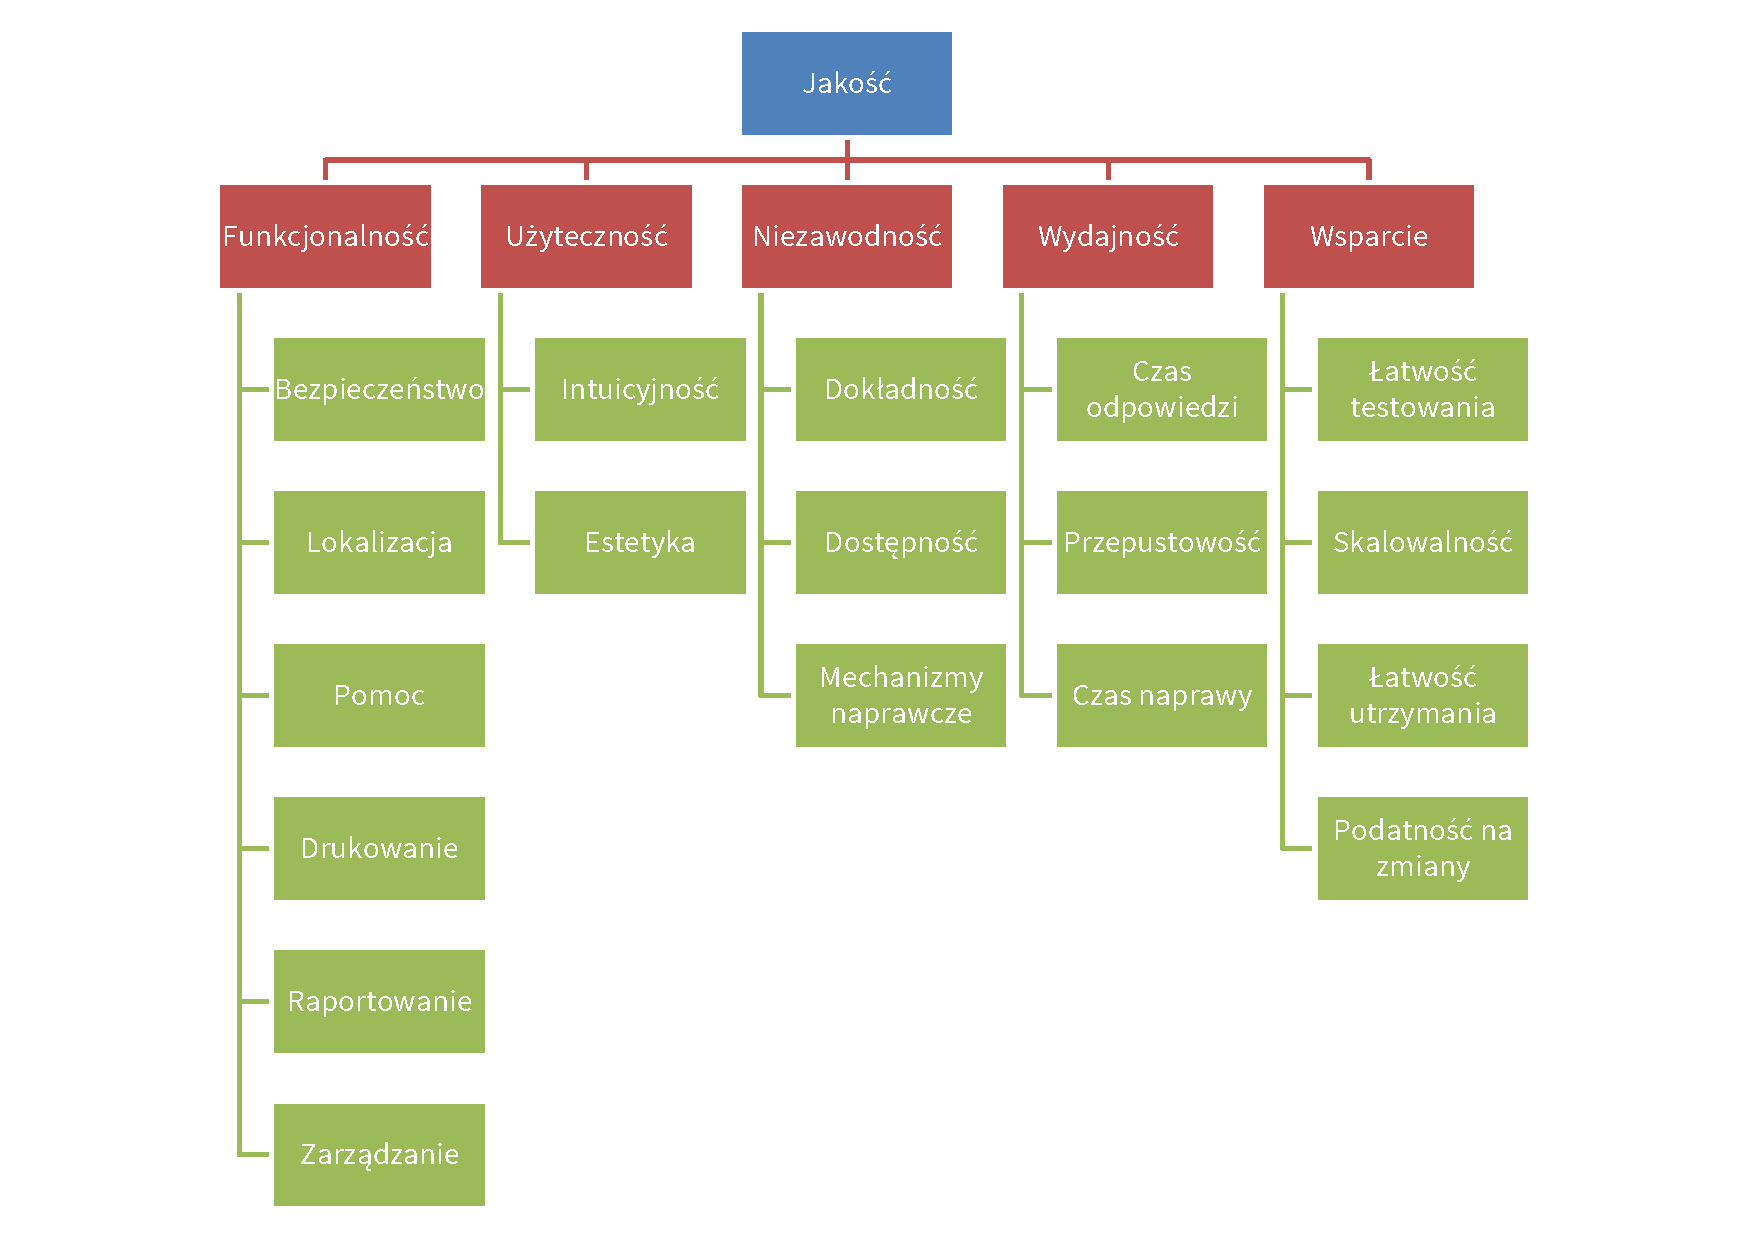
\includegraphics[trim=4cm 0cm 4cm 0cm,width=\textwidth]{./figury/schemat-do-modelu-jakosci}
    \caption{Schemat wymagań projektu \emph{Concerto}.}
    \label{fig:schemat}
\end{figure}


\newpage
\section*{Historia dokumentu}
\begin{versions}
    \version*{0.1}{2012-12-21}{ŁG}%
        Dodano opisy wymagań jakości dla produktów projektu.
    \version{0.2}{2012-12-21}{DG}%
        Dodano schemat.
    \version{0.2.1}{2012-12-22}{AO, MS}%
        Roszerzono opisy oraz metryki niektórych wymagań.
    \version{0.2.2}{2012-12-29}{ŁG}%
        Sprecyzowano metryki w wymaganiach \emph{Mechanizmy naprawcze},
        \emph{Przepustowość}, \emph{Skalowalność}.\\
    \version{1.0}{2012-12-29}{ŁG}%
        Sprawdzono. Zatwierdzono.
\end{versions}


\end{document}
